\documentclass{utap}

\usepackage{wrapfig}
\usepackage{xepersian}

\graphicspath{{./img/}}

\title{تمرین شماره‌ی ۵}
\author{
	\href{mailto:bardia.eghbali@gmail.com??subject=[AP\%20S98\%20A5]\%20}{بردیا اقبالی},
	\href{mailto:seyedahmadpourihosseini@gmail.com?subject=[AP\%20S98\%20A5]\%20}{احمد پوری‌حسینی},
	\href{mailto:ahhabibvand@gmail.com?subject=[AP\%20S98\%20A5]\%20}{امیرحسین حبیب‌وند},
	\href{mailto:farzadhabibii98@gmail.com?subject=[AP\%20S98\%20A5]\%20}{فرزاد حبیبی}
}
\course{برنامه‌سازی پیشرفته}
\lecturer{رامتین خسروی}
\deadline{جمعه ۶ اردیبهشت ۱۳۹۸، ساعت ۲۳:۵۵}

\begin{document}
	\maketitle

	\section*{ ماریو }
مقدمه
	\pagebreak

	\section{پیش‌تمرین}

در این پیش‌تمرین برنامه‌ای ساده را با کتاب‌خانۀ RSDL پیاده‌سازی می‌کنید تا بیشتر با آن آشنا شوید.


با کمک دستور draw\_img و استفاده از آرگومان src آن، می توانید تکه ای از یک تصویر را روی صفحه رسم کنید. در پوشه warmup تصویری از یک جدول 3x3 است که با اعداد 1 تا 9 پر شده. با استفاده از روش بالا برنامه ای بنویسید که به صورت تصادفی این جدول را به هم ریخته و روی صفحه رسم کند.

حالا می خواهیم با زدن دکمه R ترتیب خانه‌ها تغییر کند. برای این کار داخل یک حلقه با استفاده از تابع poll\_for\_event و get\_pressed\_key چک کنید که آیا دکمه‌ی R زده شده است یا نه. سپس مستطیل‌ها را دوباره محاسبه کنید و صفحه را بروزرسانی کنید.

تصویر زیر پنجره‌ی این برنامه را نشان می‌دهد.
	\begin{center}
		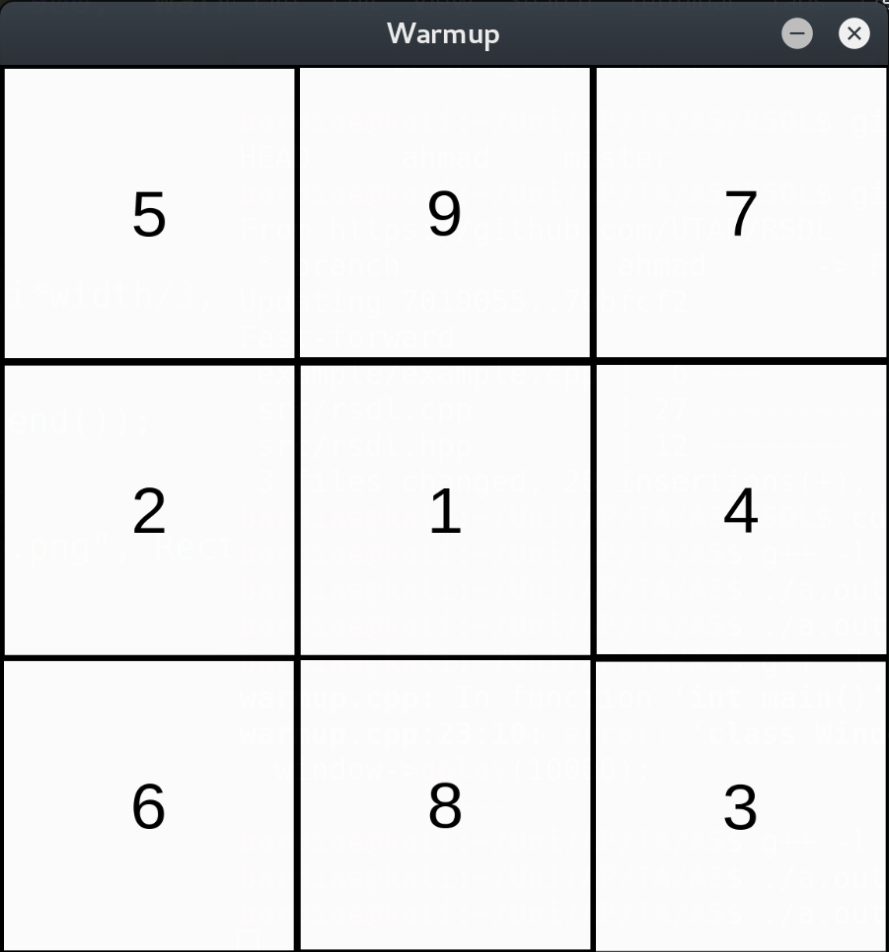
\includegraphics[width=8cm]{warmup.png}
	\end{center}
توجه کنید که این بخش برای آشنایی بیشتر شما با RSDL است و نیازی به تحویل آن نیست.
	\pagebreak

\end{document}
